\documentclass[a4paper,10pt]{report}
\usepackage[utf8]{inputenc}
\usepackage{graphicx}

% Title Page
\title{}
\author{}


\begin{document}

\section*{\textit{Layered Label Propagation Distribúido}(Esboço)}

Cada vértice terá:
\begin{itemize}
  \item A sua \textit{label}
  \item $v_i$ associado da sua $label_i$.
\end{itemize}

\begin{figure}[h]
\center
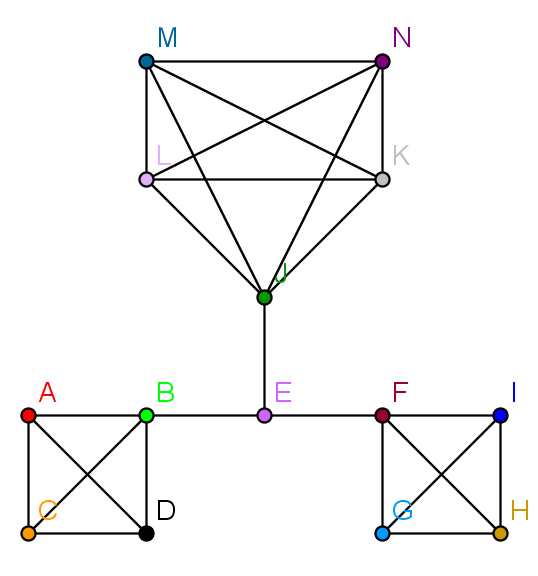
\includegraphics{graph_step0}
\caption{Primeiro grafo de exemplo.\label{fig:distributedexample1}}
\end{figure}

{\bf Exemplo para o grafo da figura \ref{fig:distributedexample1}}
\\[0.25cm]
{\bf Fase de preparação:}\\
Todos os vértices ficam com uma $label$ única. 
\\[0.25cm]
{\bf 1º \textit{Superstep}:}
Os vértices enviam para os seus adjacentes 
informação sobre a sua \textit{label} e com $v_i=1$.
\\[0.25cm]
{\bf 2º \textit{Superstep}:}
Os vértices recebem as mensagens enviadas pelos seus adjacentes e calculam a 
$label_i$ que é maximizada na sua vizinhança.
\\[0.25cm]
Vértice A:
  \begin{tabular}{| l | l | l | l |}
  \hline
  $label_i$ & $k_i$ & $v_i$ & $k_i - \gamma(v_i - k_i)$\\ \hline
  A & 0 & 1 & -1 \\ \hline
  B & 1 & 1 & 1  \\ \hline
  C & 1 & 1 & 1  \\ \hline
  D & 1 & 1 & 1  \\ \hline
  \end{tabular}
  A fica com a \textit{label} B.
\\[0.25cm]
Vértice B:
  \begin{tabular}{| l | l | l | l | l |}
  \hline
  $label_i$ & $k_i$ & $v_i$ & $k_i - \gamma(v_i - k_i)$\\ \hline
  A & 1 & 1 & 1  \\ \hline
  B & 0 & 1 & -1 \\ \hline
  C & 1 & 1 & 1  \\ \hline
  D & 1 & 1 & 1  \\ \hline
  \end{tabular}
  B fica com a \textit{label} A.
\\[0.25cm]
Vértice C:
  \begin{tabular}{| l | l | l | l |}
  \hline
  $label_i$ & $k_i$ & $v_i$ & $k_i - \gamma(v_i - k_i)$\\ \hline
  B & 1 & 1 & 1 \\ \hline
  C & 0 & 1 & -1 \\ \hline
  D & 1 & 1 & 1 \\ \hline
  \end{tabular}
  C fica com a \textit{label} A.
\\[0.25cm]
Vértice D:
  \begin{tabular}{| l | l | l | l |}
  \hline
  $label_i$ & $k_i$ & $v_i$ & $k_i - \gamma(v_i - k_i)$\\ \hline
  A & 1 & 1 & 1  \\ \hline
  B & 1 & 1 & 1  \\ \hline
  C & 1 & 1 & 1  \\ \hline
  D & 0 & 1 & -1 \\ \hline
  \end{tabular}  
  D fica com a \textit{label} A.
\\[0.25cm]
Vértice E:
  \begin{tabular}{| l | l | l | l |}
  \hline
  $label_i$ & $k_i$ & $v_i$ & $k_i - \gamma(v_i - k_i)$\\ \hline
  E & 0 & 1 & -1 \\ \hline
  B & 1 & 1 & 1  \\ \hline
  F & 1 & 1 & 1  \\ \hline
  J & 1 & 1 & 1  \\ \hline
  \end{tabular}  
  E fica com a \textit{label} B.
\\[0.25cm]
Vértice F:
  \begin{tabular}{| l | l | l | l |}
  \hline
  $label_i$ & $k_i$ & $v_i$ & $k_i - \gamma(v_i - k_i)$\\ \hline
  F & 0 & 1 & -1 \\ \hline
  E & 1 & 1 & 1  \\ \hline
  I & 1 & 1 & 1  \\ \hline
  G & 1 & 1 & 1  \\ \hline
  H & 1 & 1 & 1  \\ \hline
  \end{tabular}  
  F fica com a \textit{label} E.
\\[0.25cm]
Vértice G:
  \begin{tabular}{| l | l | l | l |}
  \hline
  $label_i$ & $k_i$ & $v_i$ & $k_i - \gamma(v_i - k_i)$\\ \hline
  G & 0 & 1 & -1  \\ \hline
  I & 1 & 1 & 1 \\ \hline
  F & 1 & 1 & 1  \\ \hline
  H & 1 & 1 & 1  \\ \hline
  \end{tabular}  
  G fica com a \textit{label} F.
\\[0.25cm]
Vértice H:
  \begin{tabular}{| l | l | l | l |}
  \hline
  $label_i$ & $k_i$ & $v_i$ & $k_i - \gamma(v_i - k_i)$\\ \hline
  H & 1 & 1 & -1  \\ \hline
  I & 0 & 1 & 1 \\ \hline
  F & 1 & 1 & 1  \\ \hline
  G & 1 & 1 & 1  \\ \hline
  \end{tabular}  
  H fica com a \textit{label} F.
\\[0.25cm]
Vértice I:
  \begin{tabular}{| l | l | l | l |}
  \hline
  $label_i$ & $k_i$ & $v_i$ & $k_i - \gamma(v_i - k_i)$\\ \hline
  I & 0 & 1 & -1 \\ \hline
  F & 1 & 1 & 1  \\ \hline
  G & 1 & 1 & 1  \\ \hline
  H & 1 & 1 & 1  \\ \hline
  \end{tabular}  
  I fica com a \textit{label} F.
\\[0.25cm]
  

  

  
\end{document}          
